% \iffalse meta-comment
%
% Copyright (C) 2015 by Josef Friedrich <josef@friedrich.rocks>
% ---------------------------------------------------------------------------
% This work may be distributed and/or modified under the
% conditions of the LaTeX Project Public License, either version 1.3
% of this license or (at your option) any later version.
% The latest version of this license is in
%   http://www.latex-project.org/lppl.txt
% and version 1.3 or later is part of all distributions of LaTeX
% version 2005/12/01 or later.
%
% This work has the LPPL maintenance status `maintained'.
%
% The Current Maintainer of this work is Josef Friedrich.
%
% This work consists of the files part-extraction.dtx and part-extraction.ins
% and the derived filebase part-extraction.sty.
%
% \fi
%
% \iffalse
%<*driver>
\ProvidesFile{part-extraction.dtx}
\documentclass{ltxdoc}
\EnableCrossrefs
\CodelineIndex
\RecordChanges
\begin{document}
  \DocInput{part-extraction.dtx}
  \PrintChanges
  \PrintIndex
\end{document}
%</driver>
%<*readme>
LaTeX/LuaLaTex class to extract parts from a full ensemble score.
%</readme>
% \fi
%
% \CheckSum{0}
%
% \CharacterTable
%  {Upper-case    \A\B\C\D\E\F\G\H\I\J\K\L\M\N\O\P\Q\R\S\T\U\V\W\X\Y\Z
%   Lower-case    \a\b\c\d\e\f\g\h\i\j\k\l\m\n\o\p\q\r\s\t\u\v\w\x\y\z
%   Digits        \0\1\2\3\4\5\6\7\8\9
%   Exclamation   \!     Double quote  \"     Hash (number) \#
%   Dollar        \$     Percent       \%     Ampersand     \&
%   Acute accent  \'     Left paren    \(     Right paren   \)
%   Asterisk      \*     Plus          \+     Comma         \,
%   Minus         \-     Point         \.     Solidus       \/
%   Colon         \:     Semicolon     \;     Less than     \<
%   Equals        \=     Greater than  \>     Question mark \?
%   Commercial at \@     Left bracket  \[     Backslash     \\
%   Right bracket \]     Circumflex    \^     Underscore    \_
%   Grave accent  \`     Left brace    \{     Vertical bar  \|
%   Right brace   \}     Tilde         \~}
%
%
% \changes{<+version+>}{<+date+>}{Converted to DTX file}
%
% \DoNotIndex{\newcommand,\newenvironment}
%
% \providecommand*{\url}{\texttt}
% \GetFileInfo{part-extraction.dtx}
% \title{The \textsf{part-extraction} package}
% \author{<+author+> \\ \url{<+email+>}}
% \date{\fileversion~from \filedate}
%
% \maketitle
%
% \section{Introduction}
%
% Put text here.
%
% \section{Usage}
%
% Put text here.
%
%
% \DescribeMacro{\partallsystems}
%
%
% \DescribeMacro{\partsystem}
%
%
% \DescribeMacro{\partsetpath}
%
%
% \DescribeMacro{\partsetextension}
%
%
% \DescribeMacro{\piece}
%
%
% \DescribeMacro{\composer}
%
%
% \StopEventually{}
%
% \section{Implementation}
%
% \iffalse
%<*package>
% \fi
%
%!TEX program = lualatex
%    \begin{macrocode}
\NeedsTeXFormat{LaTeX2e}
\ProvidesClass{part-extraction}[2015/06/19 Class to extract parts from a full ensemble score.]
\directlua{
  part = require('part-extraction')
}
\newif\ifseparator
\separatorfalse
\DeclareOption{separator}{\separatortrue}
\DeclareOption*{%
  \PassOptionsToClass{
\CurrentOption}{article}%
}
\ProcessOptions\relax
\LoadClass{article}
\RequirePackage{graphicx}
\RequirePackage[margin=1cm]{geometry}
\pagenumbering{gobble}
\setlength{\parindent}{0cm}
%    \end{macrocode}
%
% \begin{macro}{\part@system}
%    \begin{macrocode}
\newcommand{\part@system}[1]{%
  \includegraphics[width=\linewidth]{#1}%
  \ifseparator%
    \par%
    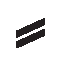
\includegraphics{separator}%
  \else%
  \fi%
    \par%
    \vfil%
}
%    \end{macrocode}
% \end{macro}
%
%
% \begin{macro}{\partallsystems}
%    \begin{macrocode}
\newcommand{\partallsystems}{%
  \directlua{
    part.print_all_systems()
  }%
  \vfill
}
%    \end{macrocode}
% \end{macro}
%
%
% \begin{macro}{\partsystem}
%    \begin{macrocode}
\newcommand{\partsystem}{%
  \directlua{
    part.print_next_system()
  }%
  \vfill
}
%    \end{macrocode}
% \end{macro}
%
%
% \begin{macro}{\partsetpath}
%    \begin{macrocode}
\newcommand{\partsetpath}[1]{\directlua{part.set_path('#1')}}
%    \end{macrocode}
% \end{macro}
%
%
% \begin{macro}{\partsetextension}
%    \begin{macrocode}
\newcommand{\partsetextension}[1]{\directlua{part.set_extension('#1')}}
%    \end{macrocode}
% \end{macro}
%
%
% \begin{macro}{\piece}
%    \begin{macrocode}
\newcommand{\piece}[1]{\def\the@piece{#1}}
%    \end{macrocode}
% \end{macro}
%
%
% \begin{macro}{\composer}
%    \begin{macrocode}
\newcommand{\composer}[1]{\def\the@composer{#1}}
%    \end{macrocode}
% \end{macro}
%
%    \begin{macrocode}
\AtBeginDocument{%
  \directlua{part.scandir()}%
  {%
  \large%
  \the@piece\
  (\the@composer)%
  }%
  \makeatletter
}
%    \end{macrocode}
%
% \iffalse
%</package>
%<*lua>
% \fi
%    \begin{macrocode}
require('lfs')

local part = {}
part.systems = {}

function part.set_path(path)
  part.path = path
end

function part.set_extension(extension)
  part.extension = extension
end

function part.scandir()
  if part.extension == nil then
    part.extension = 'png'
  end

  for filename in lfs.dir(part.path) do
    if filename:match('%.' .. part.extension .. '$') then
      table.insert(part.systems, filename)
    end
  end
end

function part.make_system(filename)
  tex.print('\\part@system{' .. part.path .. filename .. '}')
end

function part.print_all_systems()
  for key, filename in pairs(part.systems) do
    part.make_system(filename)
  end
end

function part.print_next_system()
  if not part.counter then
    part.counter = 1
  end

  part.make_system(part.systems[part.counter])

  part.counter = part.counter + 1
end

return part
%    \end{macrocode}
% \iffalse
%</lua>
% \fi
%
% \Finale
\endinput
